\documentclass[a4paper, 11pt]{article}
\setlength{\topmargin}{-0.5in}
\setlength{\textheight}{9.5in}
\setlength{\oddsidemargin}{-.1in}
\setlength{\textwidth}{6.5in}
\usepackage{graphicx}
\graphicspath{ {images/} }
\usepackage{datetime}

\begin{titlepage}

\LARGE\title{Real Time Tempo Analysis of Drum Beats}

\LARGE\author{Author: \textbf{Philip Hannant}, Supervisor: \textbf{Professor Steve Maybank}}



\end{titlepage}

\begin{document} 

\maketitle
\newpage
\tableofcontents
\clearpage

\maketitle{} \section{Introduction \& Background}
Having played the drums for nearly twenty years I have experienced a number of different training tools to help improve my timing. These tools have always been exclusive to midi driven electric drum kits, which are able to include training tools within their drum modules that use the events being triggered by the player to give live feedback on the exact timing and instrument being played. An example of such a system is the Roland DT-1 V-Drums tutor which is a software package that can be connected to a Roland V-Drum module in order to provide the player with an interactive experience that helps a drummer improve their rhythm, coordination and sight reading. Such an extensive and accurate range of tutoring functions is only made possible by the midi events that are intrinsic to an electronic drum kits function. (an example of the GUI can be found in figure 1) [1]. These tutoring tools are not however available to a drummer who does not own an electronic drum kit, such a player is restricted to using a metronome and their ear to determine their timing and rhythm. To address this, I intend to investigate the current audio tempo analysis and beat tracking algorithms available solely for the purpose of being implemented within an drum tutoring software package for the use with acoustic drums.
\begin{figure}[h]
\caption{Example of Roland DT-1 V-Drums tutor GUI}
	\centering
	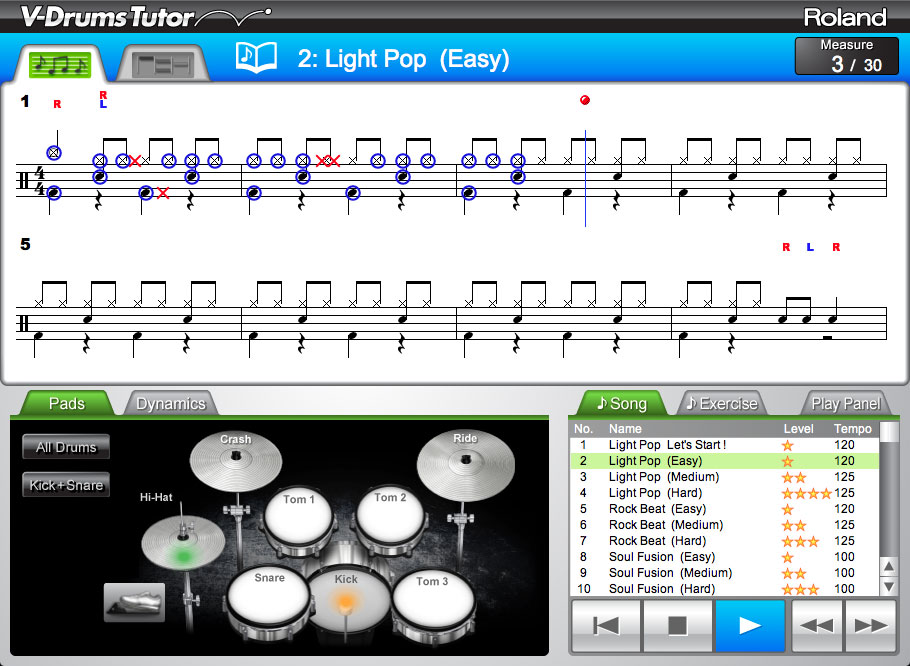
\includegraphics[scale=0.25]{dt-1_ss_main_notation_gal}
\end{figure}
\subsection{Beat Detection Background}

Detecting musical time is a skill which is not only a fundamental to musicians [2] but also something that seemingly comes naturally to humans, the majority being able to analyse and reproduce discrete metrical structures of a piece of music [3]. Producing algorithms to replicate this human ability was probably first attempted by Longuet-Higgins [2], where he began to consider that rhythm as a binary tree with each node representing a note or rest [4]. This theory developed into a system which would use a static tolerance limit on how much the downbeats varied, enabling the perceived tempo to be adjusted accordingly [2]. Since Longuet-Higgins first work there have been a number of different approaches to beat detection in audio, M. Goto and Y. Muraoka created a system which would learn the frequencies of the bass drum and snare drum, in order to then detect events triggered by these instruments during a piece of music [5]. Simon Dixon presented a system which processed a piece of audio in order to generate a tempo hypotheses at various metrical levels, multiple agents were then employed to find the sequence of beat times which best matched the salient rhythmic events which were originally detected [6].

Due to the rapidly expanding research being carried out on beat detection, in 2005 the 1st annual Music Information Retrieval Evaluation eXchange (MIREX) was held. MIREX has been set up as a contest with the goal of comparing state-of-the-art algorithms and music information retrieval [7]. The topics to be evaluated were proposed by the participants and in the first year, three of the nine topics concerned beat detection (Audio Drum Detection, Audio Onset Detection and Audio Tempo Extraction). To date, the majority beat detection software has focused mainly on the DJ industry where tempo and beat matching are popular aspects to be included in modern DJ programs. There are however other sectors of the music industry which would find beat detection software a useful, drummers in particular, would find it an enormously useful training tool.

\subsubsection{Onset Detection}
Most of the beat detection methods to date have used an onset detection function [19], the audio onset is considered to be the beginning of each music note within a piece of music[8] and therefore can be used to find time-locations within all sonic events in a piece of music [9]. 

\subsubsection{Short-Time Fourier Transform}
The Short-Time Fourier Transform (STFT) is based on the original Fourier Transform (FT) which was developed by Joseph Fourier in 1822, which can be used to find out how much of each frequency exists in a signal. The STFT was developed in order to provide a solution to the fact that the Fourier Transform does not work on non-stationary signals which results in it not being possible to used to find out when a frequency exists in the time-domain [10]. The STFT solved this issue by dividing the signal into a number smaller segments using a window function, which effectively created a series of stationary signals which the Fourier Transform could be successfully used on. This however did not fully solve the problem as the size of window function used had an effect on the the quality of frequency resolution and time resolution:
\begin{itemize}
\item Narrow Window Function $\longrightarrow$  Good Time Resolution, Bad Frequency Resolution
\item Wide Window Function $\longrightarrow$  Bad Time Resolution, Good Frequency Resolution [10]
\end{itemize}

This was eventually solved by development of the Wavelet Transforms which are capable of providing time and frequency information simultaneously in order to give a time-frequency representation of a signal, these are described in more detail in the next section.

\subsubsection{Discrete Wavelet Transform}
The Discrete Wavelet Transform (DWT) is a form of wavelet transform which foundations go back to 1976 when Crosier, Estaban and Galand devised a technique to decompose discrete time signals [11]. The DWT uses digital filtering techniques like the orginal Continuous Wavelet Transform, however it is significantly easier to implement. The DWT works by passing the signal through a series of high pass filters to analyse the high frequencies and low pass filters to do the same to low frequencies. The low pass filtering results in the resolution being halved but leaves the scale unchanged and the high filtering halves the time-resolution but doubles the frequency resolution, which effectively reduces the uncertainty in the frequency by half [11]. Due to this, the DWT is considered to share similar time-frequency resolution characteristics with the human ear [12].





\maketitle{}
\section{Aims and Objectives}

As part of my project I propose to build a real time drumbeat tempo analyser, this will use a combination of existing libraries in order to provide a basis for the creation of a live drumming tempo training tool. I will elaborate on the key features of this work in the following sections.


\subsection{Core Project Features}
\begin{itemize}
\item Adapt Eng Eder de Souza Matlab implementation of the beat tracking algorithm described by Tzanentkis, Essl and Cook [12] 
\item Record detailed comparative information regarding the efficiency and accuracy of the Beatroot and DWT implementation using JWave
\item Live audio capturing and processing
\item Build and test an extensive sample set of drum beats at varying tempos and velocities in order to ensure the system is tested against as close to a real drummer as possible
\item User interface which provides the current tempo played and notification of beat detection
\end{itemize}

\subsection{Non-Core Project Features}
\begin{itemize}
\item Create a calibration mode within the system in order to allow for the system to learn the relevant frequencies of all of the drums being played
\item Extend GUI to provide the user with real time notification on when a certain drum is played by using the stored calibrated frequencies
\end{itemize}

\maketitle{} 
\section{Development Plan for the Solution}

The main part of this project involves building a beat detection system in order to provide temporal analysis of the live audio signal. To do this I will used the Short-Time Fourier Transform based Beatroot and the algorithm described by Tzanetkis in [12] which will require the use of open source library JWave for the Discrete Wavelet Transform. 

\subsection{Beatroot}
Beatroot is an audio beat tracking system which was first presented by Simon Dixon in 2001, which he later describes as ``an off-line beat tracking system which finds the times of musical beats and tracks changes in tempo throughout a performance'' [13]. Beatroot uses two interacting processes in order to process audio; 1) Tempo induction calculated from the rate of detected beats and 2)Beat tracking produced by the synchronising the pulse sequences detected within the audio signal. These processes are performed using the following steps:

\begin{enumerate}
\item The audio signal is first passed through a onset detection function which uses the short-time Fourier transform. 
\item A clustering algorithm is then employed to find all of the significant metrical units within the signal, these clusters are then compared and ranked accordingly to produce a set of tempo hypotheses.
\item A multiple agent architecture is ultised to match the sequences of detected beats, where each agent represents a specific tempo value and alignment of beats with the audio signal.
\item Finally, the agents are evaluated against the original hypothesised beats and the highest ranked sequence is then returned as the solution.
\end{enumerate}

\subsection{JWave and Beat Detection algorithm}
JWave is a Java library created by Christian Scheiblich which provides a number different transforms including the Haar wavelets, the first DWT invented by Alfred Haar and the Daubechies wavelets, the more commonly used discrete wavelet transforms[14]. As JWave only provides the DWT component needed for this project a beat detection algorithm will need to built, which will be based on the work by Tzanetakis, Essl and Cook who described how the DWT could be used to extract information from non-speech audio, their beat detection algorithm was based on detecting the salient periodicities of the audio signal and was made up of the following steps [12]. 

\begin{enumerate}
\item Signal decomposed into a number of octave frequency bands using DWT
\item The subsequent time domain amplitude envelope is extracted for frequency each using low pass filtering, full wave rectification and downsampling
\item Each band is then normalised
\item The envelopes of each band are then summed together and an autocorrelation function is computed
\end{enumerate}

There currently is not an open source Java implementation of this algorithm, however there is a Matlab implementation of Tzanetkis, Essl \& Cook's algorithm which has been created by Eng Eder de Souza [20]. This will form the basis for the DWT based beat detection component of this project.

\subsection{Comparative analysis of Beatroot and JWave}
A key part of this project is to ascertain whether the technologies currently available are accurate enough to create a training tool similar to the midi based software described in section 1. To achieve this the 2 libraries will need to be run in parallel with the same captured audio and return details on the calculated tempo, number of beats detected and the processing speed. 

The tempo will be the beats per minute (bpm) recorded at the end of each processed frame, all of the bpm's within the sample set will be exact and in order to match the current midi software packages accuracy any returned bpm's should be exact as well. However, very small deviations in tempo can be very hard to detect to the human ear so some margin of error will be applied. To account for the fact that at the slower bpm's any beat out of place will be a lot easier to hear than at a higher bpm, the margin for error will be weighted by using the following equation;

\[ m = bpm - 60 * 0.0001\]
\begin{flushleft}
where \(m\) represents the weighted value for the margin for error to be applied.
\end{flushleft}
The data collected during this process will need to be recorded and stored in an appropriate format to allow for it to be queried and analysed at a later date. Due to the relatively small amount of data which will be collected it seems slightly excessive to create a database to do this, instead the data will be stored in a JSON file. JSON was chosen over XML as it has a much similer grammar and is able to map directly onto the data structures used in modern programming languages [21].

\subsection{Live Audio Processing}
In order to capture and process live audio the Javax Sound package will be utilised, the audio will be captured using the Java Line hierarchy; specifically the TargetDataLine class, which requires an instance of the Javax Sound AudioFormat class to be parsed in to work. The AudioFormat class is made up of a number of constructed fields which are defined as follows:

\begin{itemize}
\item Encoding - This will be set to ``''PCM.signed``'', representing audio encoded to the native linear pulse code modulation, where quantization levels are linearly uniform [15].
\item Sample Rate - 44,100, set to match CD quality for the number of analog samples which will be analysed per second. 
\item Sample Size in Bits - 24, based on a sound card with a 24 bit sample depth.
\item Channels - 2, audio will be captured using a stereo microphone.
\item Frame Size - 6, where frame size equals the number of bytes in a sample multiplied by the number of channels [17].
\item Frame Rate - 44,100, same as sample rate.
\item Big Endian (boolean) - false, as the project will be developed on an Intel core which uses a little endian architecture. Where endianess refers to the order of bytes which make up a digital word, with big endianess storing the most significant byte at a certain memory address and the remaining bytes being stored in the following higher memory addresses. The little-endian formate reverses the order storing the least significant at the lowest and most significant at the highest memory address [16].
\end{itemize}


\subsection{Build Extensive drum sample set}
The success of this project will rely heavily on the amount of data that the system can produce and in order to do this a large set of drum beat samples will need to be created. The drum beats themselves will be created using the midi drumbeats within the Apple software package, Garageband. The sample set will need to contains beats from a variety of styles as well as samples with fluctuating tempos. The main aspects of the sample set can be found below:

\begin{itemize}
\item The tempo range will be 60 - 160 beats per minute, although some samples will be be created with varying tempos in order to closely reflect a real human player
\item The time signatures will be mainly in common time (4/4) to reflect playing styles, however some beats will use swing time which will either be created by feel within the sample or by using triplets with a duple meter in 12/8
\item Velocities will be varied across the sample set, accent and ghost notes will be used in line with a real playing style
\item The sample set will contain a wide range of drum beats, including; beats using one drum, those only with a back beat, beats incorporating single rests within a bar or for the whole duration of a bar and beats with large solos \& cymbal work
\end{itemize} 

Musical styles will comprise of rock \& pop, blues and jazz, with the main emphasis failing on rock \& pop beats. Each style will have between 5 - 10 unique samples created, which will in turn each be sampled with a bpm value starting at 60 and increasing in steps of 5 up until the maximum 160. This will account for approximately 500 separate samples. There will also be a final set of simple single and multiple drum beats included which will produce another c. 10 unique samples, which will give a total sample set size of c. 750 samples.

\subsection{Develop User Interface}
The user interface will be developed using the JavaFX framework, which will ensure that the system will be cross-platform compatible. It's features will be kept simple initially as it will only be required to display the current two tempo calculations and accumulative count of beats detected.

\subsection{Non-Core Project Features}
The inclusion of the non-core project features will only occur if the project is developed ahead of the predetermined schedule described in section 4. 

\subsubsection{Calibration Mode}
Like in the system developed by Goto and Muraoka, which learnt the frequencies of the snare and kick drum in order to detect events triggered by these instruments [5]. This additional feature of the project will look to create a mode in the system which can be used to detect and record the frequencies of all of the parts of a drum kit (snare, kick, tom toms, hi-hat and cymbals).

\subsubsection{Extend User Interface}
This feature will look to recreate the Roland DT-1 user interface seen in figure 1 and developing this additional feature will only be possible if the calibration mode has been successfully developed. The user interface will look to recreate the drum kit visual seen in figure 1, where a colour indicator will be displayed to represent whether the players last hit was in time. The development of this final feature depends heavily on the accuracy and efficiency of the tempo analysis algorithms used.

\subsection{Project Methodology}
The development of this project will be carried out using the Test Driven Development (TDD) framework, TDD is a development process that is made up of a very short development cycles. First a failing automated test is developed, then the minimum of code is written to pass this test, finally, the code is refactored accordingly in order to produce code at the appropriate standard [18].

\subsection{Development Languages and Testing}
The project will developed in a combination of Java and Scala. Java is required as both the Beatroot and JWave libraries are in this language, however any functional aspects of the project will be developed in Scala, as it offers a superior functional tool set when compared to those offered in Java 8. As previously discussed JSON will be used to store the collected data.
I will use the Intellij IDE to develop this system, Git will be used for version control and testing will be completed using JUnit for Java and Scala Test for any functionality developed in Scala. In order to ensure that the parsed JSON is well formed it will be tested using the JSON validator found at - http://jsonlint.com/.

\clearpage
\maketitle{} 
\section {Project Schedule}
The start date for the project is Monday 13th June 2016 and the end date is Monday 19th September 2016, the non-core project features will only be completed if the project is ahead of schedule.
\begin{table}[h]
\caption{Project Timeline} 
\centering
\begin{tabular}{|p{4cm}|p{8cm}|}
 \hline
\textbf{Dates} & \textbf{Task}\\ [0.5ex]
\hline 
w/c 13th June 2016 & Develop live audio capturing system\\
\hline 
w/c 20th June 2016 & Set up Beatroot library in development environment\\
\hline 
w/c 27th June 2016 & Implement DWT tempo and beat detection algorithm in Scala/Java\\
\hline 
w/c 4th July 2016 & Test systems with single live audio source\\
\hline 
w/c 11th July 2016 & Develop system to store data generated during tempo analysis\\
\hline 
w/c 18th July 2016 & Research and build appropriate framework to process captured audio in parallel e.g. akka actors\\
\hline 
w/c 1st August 2016 & Create sample set of drum beats\\
\hline 
w/c 8th August 2016 & Test system using full sample set\\
\hline 
w/c 15th August 2016 & Develop UI\\
\hline 
w/c 22nd August 2016 & Analyse logged data\\
\hline 
w/c 29th August 2026 & Write up report\\
\hline 
w/c 5th September 2016 & Present findings to project supervisor\\
\hline 
w/c 12th September 2016 & Finalise report\\
\hline 
w/c 19th September 2016 & Submit report\\
\hline
\end{tabular}
\end{table}
\clearpage
\maketitle{} 
\section{Conclusion}
I have proposed to build a real-time drumbeat tempo analysis system using the Short-Time Fourier Transform based Beatroot library and an implementation of the beat detection algorithm using Discrete Wavelet Transforms developed by Tzanetkis et al. In order to ascertain how close these systems are to being able to replicate the training tools currently available to drummers on electric drum kits.


\maketitle{} 
\section{References}
\begin{enumerate}
\item http://www.roland.co.uk/blog/exploring-roland-dt-1-v-drums-tutor-software/
\item Allen and Dannenberg (1990), Tracking Musical Beats in Real Time, International Computer Music Conference, International Computer Music Association, pp. 140-143
\item P. Desain and H. Honing (1989), The Quantization of Musical Time: A Connectionist Approach, Computer Music Journal, Vol. 13 No. 3 (Autumn), pp. 56-66
\item H. C Longuet-Higgins (1976), Perception of melodies, Nature Vol. 263, pp. 646-653
\item M. Goto and Y. Muraoka (1994), A beat tracking system for acoustic signals of music, in Proceedings of the Second ACM International Conference on Multimedia, pp. 365-372
\item S. Dixon (2001), Automatic Extraction of Tempo and Beat from Expressive Performances, Journal of New Music Research, 30 (1), pp. 39-58.
\item http://www.music-ir.org/mirex/wiki/2005:Main\_Page
\item https://en.wikipedia.org/wiki/Onset\_(audio)
\item http://www.music-ir.org/mirex/wiki/2016:Audio\_Onset\_Detection
\item http://users.rowan.edu/~polikar/WAVELETS/WTpart2.html
\item http://users.rowan.edu/~polikar/WAVELETS/WTpart4.html
\item G. Tzanetakis, G. Essl and P. Cook (2001), Audio Analysis using the Discrete Wavelet Transform, Proc. WSES International Conference on Acoustics and Music: Theory and Applications (AMTA)
\item S. Dixon (2003), On the Analysis of Musical Expression in Audio Signals, Storage and Retrieval for Media Databases, SPIE-IS\&T Electronic Imaging, SPIE Vol. 5021, pp. 122-132
\item https://en.wikipedia.org/wiki/Discrete\_wavelet\_transform
\item https://en.wikipedia.org/wiki/Pulse-code\_modulation
\item https://en.wikipedia.org/wiki/Endianness
\item http://www.jsresources.org/faq\_audio.html
\item https://en.wikipedia.org/wiki/Test-driven\_development
\item A. Robertson, A. Stark and M. E. P. Davies (2013), Percussive Beat tracking using real-time median filtering, 6th International Workshop on Machine Learning and Music
\item https://github.com/ederwander/Beat-Track
\item http://www.json.org/xml.html
\end{enumerate}
\end{document}
